
The local memory interconnect is responsible for routing requests from the
CPU to the appropriate peripheral.
It also enforces the first stage of the SoC memory map.

\begin{figure}
\centering
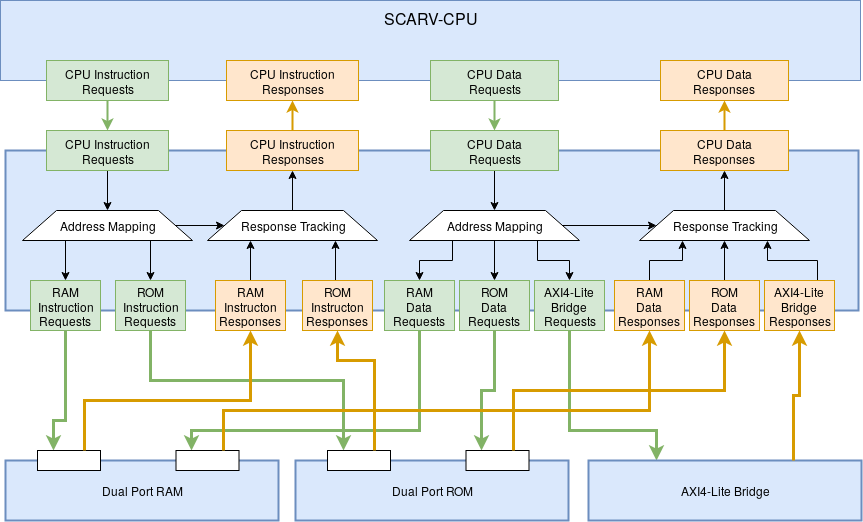
\includegraphics[width=0.8\textwidth]{image/soc-local-ic.png}
\caption{
Block diagram of the \SCARVSOC inner sub-system memory interconnect, 
showing how the \SCARVCPU instruction and data memory requests/responses
are routed to each peripheral.
}
\label{fig:design:soc-local-ic}
\end{figure}

\noindent Input Request Ports:
\begin{enumerate}

\item CPU instruction fetch interface. Reads only.

\item CPU data interface. Reads and Writes. Writes are non-posted.

\end{enumerate}


\noindent Output request ports:
\begin{enumerate}

\item Boot ROM (Instructions)

\item Boot ROM (Data)

\item RAM (Instructions)

\item RAM (Data)

\item AXI port (Data Only).

\end{enumerate}

All local RAM/ROM accesses have 1 cycle access latency.

The AXI port is optimised for low resource usage and simplicity.
All requests block until they are completed. There is no
tracking of outstanding requests.
All AXI requests have a minimum 2 cycle latency for reads and writes.

The local interconnect is responsible for returning error responses
when a request is made to unmapped addresses.
This is done using a {\em stub} peripheral, which unmapped address
requests are always routed too.
The stub peripheral then always returns an error response.
There is a single stub peripheral for each CPU requestor interface.

